\documentclass{ximera}


\graphicspath{
  {./}
  {ximeraTutorial/}
  {basicPhilosophy/}
}

\newcommand{\mooculus}{\textsf{\textbf{MOOC}\textnormal{\textsf{ULUS}}}}


\usepackage{tkz-euclide}\usepackage{tikz}
\usepackage{tikz-cd}
\usetikzlibrary{arrows}
\tikzset{>=stealth,commutative diagrams/.cd,
  arrow style=tikz,diagrams={>=stealth}} %% cool arrow head
\tikzset{shorten <>/.style={ shorten >=#1, shorten <=#1 } } %% allows shorter vectors

\usetikzlibrary{backgrounds} %% for boxes around graphs
\usetikzlibrary{shapes,positioning}  %% Clouds and stars
\usetikzlibrary{matrix} %% for matrix
\usepgfplotslibrary{polar} %% for polar plots
\usepgfplotslibrary{fillbetween} %% to shade area between curves in TikZ
\usetkzobj{all}
\usepackage[makeroom]{cancel} %% for strike outs
%\usepackage{mathtools} %% for pretty underbrace % Breaks Ximera
%\usepackage{multicol}
\usepackage{pgffor} %% required for integral for loops



%% http://tex.stackexchange.com/questions/66490/drawing-a-tikz-arc-specifying-the-center
%% Draws beach ball
\tikzset{pics/carc/.style args={#1:#2:#3}{code={\draw[pic actions] (#1:#3) arc(#1:#2:#3);}}}



\usepackage{array}
\setlength{\extrarowheight}{+.1cm}
\newdimen\digitwidth
\settowidth\digitwidth{9}
\def\divrule#1#2{
\noalign{\moveright#1\digitwidth
\vbox{\hrule width#2\digitwidth}}}
























%%This is to help with formatting on future title pages.
\newenvironment{sectionOutcomes}{}{}


\title{Similarity}

\begin{document}

\begin{abstract}
unit circle again
\end{abstract}
\maketitle



\begin{itemize}
\item The position of \textbf{every} point in the Cartesian plane can be described as a scalar times a direction vector.  A direction vector has unit length.

\item \textbf{Every} Complex number can be represented as the product of a real number and a complex number with modulus $1$.


\item \textbf{Every} Complex number can be represented as the product of a real number and a complex number that sits on the unit circle.
\end{itemize}








\begin{image}
\begin{tikzpicture}
  \begin{axis}[
            xmin=-1.1,xmax=1.1,ymin=-1.1,ymax=1.1,
            axis lines=center,
            width=4in,
            xtick={-1,1},
            ytick={-1,1},
            clip=false,
            unit vector ratio*=1 1 1,
            xlabel=$x$, ylabel=$y$,
            ticklabel style={font=\scriptsize},
            every axis y label/.style={at=(current axis.above origin),anchor=south},
            every axis x label/.style={at=(current axis.right of origin),anchor=west},
          ]        
          \addplot [smooth, domain=(0:360)] ({cos(x)},{sin(x)}); %% unit circle

          \addplot [textColor] plot coordinates {(0,0) (.766,.643)}; %% 40 degrees

          \addplot [ultra thick,penColor] plot coordinates {(.766,0) (.766,.643)}; %% 40 degrees
          \addplot [ultra thick,penColor2] plot coordinates {(0,0) (.766,0)}; %% 40 degrees
          
          %\addplot [ultra thick,penColor3] plot coordinates {(1,0) (1,.839)}; %% 40 degrees          

          \addplot [textColor,smooth, domain=(0:40)] ({.15*cos(x)},{.15*sin(x)});
          %\addplot [very thick,penColor] plot coordinates {(0,0) (.766,.643)}; %% sector
          %\addplot [very thick,penColor] plot coordinates {(0,0) (1,0)}; %% sector
          %\addplot [very thick, penColor, smooth, domain=(0:40)] ({cos(x)},{sin(x)}); %% sector
          \node at (axis cs:.15,.07) [anchor=west] {$\theta$};
          \node[penColor, rotate=-90] at (axis cs:.84,.322) {$\sin(\theta)$};
          \node[penColor2] at (axis cs:.383,0) [anchor=north] {$\cos(\theta)$};
          %\node[penColor3, rotate=-90] at (axis cs:1.06,.322) {$\tan(\theta)$};

          \addplot[color=black,fill=black,only marks,mark=*] coordinates{(0.766,0.643)}; 

        \end{axis}
\end{tikzpicture}
\end{image}







\begin{theorem} \textbf{\textcolor{green!50!black}{Complex Multiplication (Polar Form)}}  

\[  (r_1, \theta_1) \cdot (r_2, \theta_2) = (r_1 \cdot r_2, \theta_1 + \theta_2)              \]


\end{theorem}




To understand the Complex numbers, we just need to understand the unit circle.  To understand the unit circle, we just need to understand right triangles.







\section{Right Triangles}




$\blacktriangleright$ \textbf{Similar Triangles} \\

From Geometry, we know that triangles with the same three angles are called \textbf{similar}.  Similar triangles can be of different sizes, but their sides are always proportional.







$\blacktriangleright$ \textbf{Unit Circle} \\




If we pick $\theta$, then we have defined a right triangle via the unit circle.









\begin{image}
\begin{tikzpicture}
  \begin{axis}[
            xmin=-1.1,xmax=1.1,ymin=-1.1,ymax=1.1,
            axis lines=center,
            width=4in,
            xtick={-1,1},
            ytick={-1,1},
            clip=false,
            unit vector ratio*=1 1 1,
            xlabel=$x$, ylabel=$y$,
            ticklabel style={font=\scriptsize},
            every axis y label/.style={at=(current axis.above origin),anchor=south},
            every axis x label/.style={at=(current axis.right of origin),anchor=west},
          ]        
          \addplot [smooth, domain=(0:360)] ({cos(x)},{sin(x)}); %% unit circle

          \addplot [textColor] plot coordinates {(0,0) (.766,.643)}; %% 40 degrees

          \addplot [ultra thick,penColor] plot coordinates {(.766,0) (.766,.643)}; %% 40 degrees
          \addplot [ultra thick,penColor2] plot coordinates {(0,0) (.766,0)}; %% 40 degrees
          
          %\addplot [ultra thick,penColor3] plot coordinates {(1,0) (1,.839)}; %% 40 degrees          

          \addplot [textColor,smooth, domain=(0:40)] ({.15*cos(x)},{.15*sin(x)});
          %\addplot [very thick,penColor] plot coordinates {(0,0) (.766,.643)}; %% sector
          %\addplot [very thick,penColor] plot coordinates {(0,0) (1,0)}; %% sector
          %\addplot [very thick, penColor, smooth, domain=(0:40)] ({cos(x)},{sin(x)}); %% sector
          \node at (axis cs:.15,.07) [anchor=west] {$\theta$};
          \node[penColor, rotate=-90] at (axis cs:.84,.322) {$\sin(\theta)$};
          \node[penColor2] at (axis cs:.383,0) [anchor=north] {$\cos(\theta)$};
          %\node[penColor3, rotate=-90] at (axis cs:1.06,.322) {$\tan(\theta)$};

          \addplot[color=black,fill=black,only marks,mark=*] coordinates{(0.766,0.643)}; 

        \end{axis}
\end{tikzpicture}
\end{image}





The hypotenuse is the radius of the circle, which has a length of $1$.

By extending the radius to larger circles we can create many right triangles.  As long as the angle stays the same, then we have similar triangles and all of the sides are proportional.



\begin{image}[3in]
    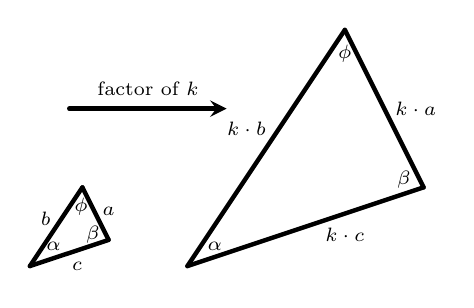
\begin{tikzpicture}[line cap=round]



  \draw [ultra thick] (0,0) -- (3,1);
  \draw [ultra thick] (3,1) -- (2,3);
  \draw [ultra thick] (0,0) -- (2,3);

  \draw [rotate=0] (0.35,0.25) node {\scriptsize{$\alpha$}};
  \draw [rotate=0] (2.75,1.1) node {\scriptsize{$\beta$}};
  \draw [rotate=0] (2,2.7) node {\scriptsize{$\phi$}};

  \draw (-1.4,0) node {\scriptsize{$c$}};
  \draw (-1,0.7) node {\scriptsize{$a$}};
  \draw (-1.8,0.6) node {\scriptsize{$b$}};





  \draw [ultra thick] (-2,0) -- (-1,0.333);
  \draw [ultra thick] (-1,0.333) -- (-1.333,1);
  \draw [ultra thick] (-2,0) -- (-1.333,1);

  \draw [rotate=0] (-1.7,0.25) node {\scriptsize{$\alpha$}};
  \draw [rotate=0] (-1.2,0.4) node {\scriptsize{$\beta$}};
  \draw [rotate=0] (-1.35,0.75) node {\scriptsize{$\phi$}};

  \draw (2.9,2) node {\scriptsize{$k \cdot a$}};
  \draw (0.75,1.75) node {\scriptsize{$k \cdot b$}};
  \draw (2,0.4) node {\scriptsize{$k \cdot c$}};


  \draw [ultra thick,->] (-1.5,2) -- (0.5,2);
  \draw [rotate=0] (-0.5,2.25) node {\scriptsize{factor of $k$}};










    \end{tikzpicture}
  \end{image}


We can use this to extend our right triangles on the unit circle outward into the Complex Plane. \\










\section{Right Triangles}



Since our initial right triangle was anchored to the unit circle, its hypotenuse has length $1$.  The hypotenuses of the other similar right triangles have a length, which we'll call $r$.



\begin{image}
\begin{tikzpicture}
  \begin{axis}[
            xmin=-5,xmax=5,ymin=-5,ymax=5,
            axis lines=center,
            width=4in,
            xtick={-4,-3,-2,-1,1,2,3,4},
            ytick={-4,-3,-2,-1,1,2,3,4},
            clip=false,
            unit vector ratio*=1 1 1,
            xlabel=$x$, ylabel=$y$,
            ticklabel style={font=\scriptsize},
            every axis y label/.style={at=(current axis.above origin),anchor=south},
            every axis x label/.style={at=(current axis.right of origin),anchor=west},
          ]        
          \addplot [smooth, domain=(0:360)] ({cos(x)},{sin(x)}); %% unit circle

          \addplot [textColor] plot coordinates {(0,0) (.766,.643)}; %% 40 degrees

          \addplot [ultra thick,penColor] plot coordinates {(.766,0) (.766,.643)}; %% 40 degrees
          \addplot [ultra thick,penColor2] plot coordinates {(0,0) (.766,0)}; %% 40 degrees
          
          %\addplot [ultra thick,penColor3] plot coordinates {(1,0) (1,.839)}; %% 40 degrees          

          \addplot [textColor,smooth, domain=(0:40)] ({.15*cos(x)},{.15*sin(x)});
          %\addplot [very thick,penColor] plot coordinates {(0,0) (.766,.643)}; %% sector
          %\addplot [very thick,penColor] plot coordinates {(0,0) (1,0)}; %% sector
          %\addplot [very thick, penColor, smooth, domain=(0:40)] ({cos(x)},{sin(x)}); %% sector
          \node at (axis cs:.15,.25) [anchor=west] {\scriptsize{$\theta$}};
          %\node[penColor, rotate=-90] at (axis cs:.84,.322) {$\scriptsize{\sin(\theta)}$};
          %\node[penColor2] at (axis cs:.383,0) [anchor=north] {$\cos(\theta)$};
          %\node[penColor3, rotate=-90] at (axis cs:1.06,.322) {$\tan(\theta)$};

          \addplot [textColor] plot coordinates {(0,0) (1.915,1.607)}; %% 40 degrees
          \addplot [ultra thick,penColor] plot coordinates {(1.915,0) (1.915,1.607)}; %% 40 degrees
          \addplot [ultra thick,penColor2] plot coordinates {(0,0) (1.915,0)}; %% 40 degrees

          \addplot [textColor] plot coordinates {(0,0) (2.681,2.250)}; %% 40 degrees
          \addplot [ultra thick,penColor] plot coordinates {(2.681,0) (2.681,2.250)}; %% 40 degrees
          \addplot [ultra thick,penColor2] plot coordinates {(0,0) (2.681,0)}; %% 40 degrees
          
          


        \end{axis}
\end{tikzpicture}
\end{image}










\begin{image}
\begin{tikzpicture}
  \begin{axis}[
            xmin=-2.1,xmax=2.1,ymin=-2.1,ymax=2.1,
            axis lines=center,
            width=4in,
            xtick={-2,-1,1,2},
            ytick={-2,-1,1,2},
            clip=false,
            unit vector ratio*=1 1 1,
            xlabel=$x$, ylabel=$y$,
            ticklabel style={font=\scriptsize},
            every axis y label/.style={at=(current axis.above origin),anchor=south},
            every axis x label/.style={at=(current axis.right of origin),anchor=west},
          ]        
          \addplot [smooth, domain=(0:360)] ({cos(x)},{sin(x)}); %% unit circle

          \addplot [textColor] plot coordinates {(0,0) (.766,.643)}; %% 40 degrees

          \addplot [ultra thick,penColor] plot coordinates {(.766,0) (.766,.643)}; %% 40 degrees
          \addplot [ultra thick,penColor2] plot coordinates {(0,0) (.766,0)}; %% 40 degrees
          
          %\addplot [ultra thick,penColor3] plot coordinates {(1,0) (1,.839)}; %% 40 degrees          

          \addplot [textColor,smooth, domain=(0:40)] ({.15*cos(x)},{.15*sin(x)});
          %\addplot [very thick,penColor] plot coordinates {(0,0) (.766,.643)}; %% sector
          %\addplot [very thick,penColor] plot coordinates {(0,0) (1,0)}; %% sector
          %\addplot [very thick, penColor, smooth, domain=(0:40)] ({cos(x)},{sin(x)}); %% sector
          \node at (axis cs:.15,.1) [anchor=west] {\scriptsize{$\theta$}};
          %\node[penColor, rotate=-90] at (axis cs:.84,.322) {$\sin(\theta)$};
          %\node[penColor2] at (axis cs:.383,0) [anchor=north] {$\cos(\theta)$};
          %\node[penColor3, rotate=-90] at (axis cs:1.06,.322) {$\tan(\theta)$};




          \addplot [smooth, domain=(0:360)] ({1.7*cos(x)},{1.7*sin(x)}); 

          \addplot [textColor] plot coordinates {(0,0) (1.3,1.09)}; %% 40 degrees

          \addplot [ultra thick,penColor] plot coordinates {(1.3,0) (1.3,1.09)}; %% 40 degrees
          \addplot [ultra thick,penColor2] plot coordinates {(0,0) (1.3,0)}; %% 40 degrees

          \node[penColor, rotate=-90] at (axis cs:1.45,.5) {$r \sin(\theta)$};
          \node[penColor2] at (axis cs:.85,0) [anchor=north] {$r \cos(\theta)$};


          \node at (axis cs:.8,.9) [anchor=west] {$r$};

          \addplot[color=black,fill=black,only marks,mark=*] coordinates{(0.766,0.643)}; 


        \end{axis}
\end{tikzpicture}
\end{image}



The two right triangles are similar.  

The ratio of corresponding sides are equal.











\begin{image}[3in]
    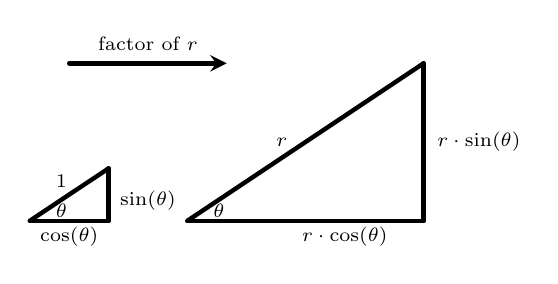
\begin{tikzpicture}[line cap=round]



  \draw [ultra thick] (0,0) -- (3,0);
  \draw [ultra thick] (3,0) -- (3,2);
  \draw [ultra thick] (0,0) -- (3,2);

  \draw [rotate=0] (0.4,0.13) node {\scriptsize{$\theta$}};


  \draw (3.05,1) node  [anchor=west]{\scriptsize{$r \cdot \sin(\theta)$}};
  \draw (1.2,1) node {\scriptsize{$r$}};
  \draw (2,-0.2) node {\scriptsize{$r \cdot \cos(\theta)$}};





  \draw [ultra thick] (-2,0) -- (-1,0);
  \draw [ultra thick] (-1,0) -- (-1,0.666);
  \draw [ultra thick] (-2,0) -- (-1,0.666);

  \draw [rotate=0](-1.6,0.13) node {\scriptsize{$\theta$}};





  \draw (-0.5,0.25) node {\scriptsize{$\sin(\theta)$}};
  \draw (-1.5,-0.2) node {\scriptsize{$\cos(\theta)$}};
  \draw (-1.6,0.5) node {\scriptsize{$1$}};


  \draw [ultra thick,->] (-1.5,2) -- (0.5,2);
  \draw [rotate=0] (-0.5,2.25) node {\scriptsize{factor of $r$}};










    \end{tikzpicture}
  \end{image}









This has to be true for any right triangle with an angle $\theta$.

If we label the sides relative to the angle $\theta$, then we obtain descriptive ratios.


\begin{image}[3in]
    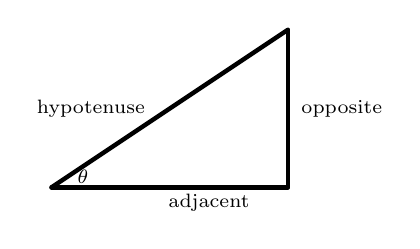
\begin{tikzpicture}[line cap=round]



  \draw [ultra thick] (0,0) -- (3,0);
  \draw [ultra thick] (3,0) -- (3,2);
  \draw [ultra thick] (0,0) -- (3,2);

  \draw [rotate=0] (0.4,0.13) node {\scriptsize{$\theta$}};


  \draw (3.05,1) node  [anchor=west]{\scriptsize{opposite}};
  \draw (0.5,1) node {\scriptsize{hypotenuse}};
  \draw (2,-0.2) node {\scriptsize{adjacent}};







    \end{tikzpicture}
  \end{image}


The ratios have to be the same as for the unit circle triangle.


\[   \sin(\theta) = \frac{opp}{hyp}           \]



\[   \cos(\theta) = \frac{adj}{hyp}           \]




\[   \tan(\theta) = \frac{\sin(\theta)}{\cos(\theta)}    = \frac{opp}{adj}        \]








\section{Other Quadrants}


Everything holds for larger angles.  We just have to bridge two thoughts.  


\begin{itemize}
\item The coordinates of points might be negative.  
\item Lengths of sides of triangles are not negative.
\end{itemize}

To help bridge these two thoughts we will have two angles and two triangles.  


\begin{itemize}
\item The actual angle, $\theta$, roatating from the positive $x$-axis.  
\item The \textbf{reference angle}, $\phi$, which will sit inside our reference triangle formed with the horizontal axis.
\end{itemize}





\begin{image}
\begin{tikzpicture}
  \begin{axis}[
            xmin=-2.1,xmax=2.1,ymin=-2.1,ymax=2.1,
            axis lines=center,
            width=4in,
            xtick={-2,1,2},
            ytick={-2,-1,1,2},
            clip=false,
            unit vector ratio*=1 1 1,
            xlabel=$x$, ylabel={Quadrant II},
            ticklabel style={font=\scriptsize},
            every axis y label/.style={at=(current axis.above origin),anchor=south},
            every axis x label/.style={at=(current axis.right of origin),anchor=west},
          ]        
          \addplot [smooth, domain=(0:360)] ({cos(x)},{sin(x)}); %% unit circle

          %\addplot [textColor] plot coordinates {(0,0) (.766,.643)}; %% 40 degrees

          %\addplot [ultra thick,penColor] plot coordinates {(.766,0) (.766,.643)}; %% 40 degrees
          %\addplot [ultra thick,penColor2] plot coordinates {(0,0) (.766,0)}; %% 40 degrees
          
          %\addplot [ultra thick,penColor3] plot coordinates {(1,0) (1,.839)}; %% 40 degrees          

          \addplot [textColor,smooth, domain=(0:140)] ({.15*cos(x)},{.15*sin(x)});
          %\addplot [very thick,penColor] plot coordinates {(0,0) (.766,.643)}; %% sector
          %\addplot [very thick,penColor] plot coordinates {(0,0) (1,0)}; %% sector
          %\addplot [very thick, penColor, smooth, domain=(0:40)] ({cos(x)},{sin(x)}); %% sector
          \node at (axis cs:.05,.15) [anchor=west] {\scriptsize{$\theta$}};
          %\node[penColor, rotate=-90] at (axis cs:.84,.322) {$\sin(\theta)$};
          %\node[penColor2] at (axis cs:.383,0) [anchor=north] {$\cos(\theta)$};
          %\node[penColor3, rotate=-90] at (axis cs:1.06,.322) {$\tan(\theta)$};




          \addplot [smooth, domain=(0:360)] ({1.7*cos(x)},{1.7*sin(x)}); 
          \addplot [textColor,smooth, domain=(140:180)] ({.19*cos(x)},{.19*sin(x)});
          \node at (axis cs:-0.2,.15) [anchor=east] {\scriptsize{$\phi$}};

          \addplot [textColor] plot coordinates {(0,0) (-1.3,1.09)}; %% 40 degrees

          \addplot [ultra thick,penColor] plot coordinates {(-1.3,0) (-1.3,1.09)}; %% 40 degrees
          \addplot [ultra thick,penColor2] plot coordinates {(0,0) (-1.3,0)}; %% 40 degrees

          \node[penColor, rotate=-90] at (axis cs:-1.45,.5) {$r \sin(\phi)$};
          \node[penColor2] at (axis cs:-.85,0) [anchor=north] {$r \cos(\phi)$};


          \node at (axis cs:-0.8,.8) [anchor=west] {$r$};



           \node[penColor2] at (axis cs:-1.3,1.2) [anchor=east] {$( r \cos(\theta), $};
           \node[penColor] at (axis cs:-1.3,1.2) [anchor=west] {$r \sin(\theta) ) $};

           \addplot[color=black,fill=black,only marks,mark=*] coordinates{(-1.3,1.09)}; 


        \end{axis}
\end{tikzpicture}
\end{image}




Once we rotate out of the first quadrant, then we need to switch our visual right triangle. \\


If $\theta$ is in the second quadrant, then we use a new right triangle formed with the $x$-axis. $\theta$ sweeps out to our hypotenuse, however, $\theta$ is no longer inside our reference right triangle.  Instead we have the angle $\phi = \pi - \theta$.  

The point at the end of our hypotenuse has coordinates, $(\cos(\theta), \sin(\theta))$.  In the second quadrant, these coordinates are negative and positive: $\cos(\theta) < 0$ and $\sin(\theta) > 0$.

However, practically speaking, we use the reference angle and reference triangle to calculate values.  After calculating the lengths of the sides of the reference triangle, we must remember to change their signs appropriately. 


\begin{example} Quadrant II \\




\begin{image}
\begin{tikzpicture}
  \begin{axis}[
            xmin=-2.1,xmax=2.1,ymin=-2.1,ymax=2.1,
            axis lines=center,
            width=4in,
            xtick={-2,1,2},
            ytick={-2,-1,1,2},
            clip=false,
            unit vector ratio*=1 1 1,
            xlabel=$x$, ylabel={Quadrant II},
            ticklabel style={font=\scriptsize},
            every axis y label/.style={at=(current axis.above origin),anchor=south},
            every axis x label/.style={at=(current axis.right of origin),anchor=west},
          ]        
          \addplot [smooth, domain=(0:360)] ({cos(x)},{sin(x)}); %% unit circle

          %\addplot [textColor] plot coordinates {(0,0) (.766,.643)}; %% 40 degrees

          %\addplot [ultra thick,penColor] plot coordinates {(.766,0) (.766,.643)}; %% 40 degrees
          %\addplot [ultra thick,penColor2] plot coordinates {(0,0) (.766,0)}; %% 40 degrees
          
          %\addplot [ultra thick,penColor3] plot coordinates {(1,0) (1,.839)}; %% 40 degrees          

          \addplot [textColor,smooth, domain=(0:140)] ({.15*cos(x)},{.15*sin(x)});
          %\addplot [very thick,penColor] plot coordinates {(0,0) (.766,.643)}; %% sector
          %\addplot [very thick,penColor] plot coordinates {(0,0) (1,0)}; %% sector
          %\addplot [very thick, penColor, smooth, domain=(0:40)] ({cos(x)},{sin(x)}); %% sector
          \node at (axis cs:.05,.15) [anchor=west] {\scriptsize{$\tfrac{3 \pi}{4}$}};
          %\node[penColor, rotate=-90] at (axis cs:.84,.322) {$\sin(\theta)$};
          %\node[penColor2] at (axis cs:.383,0) [anchor=north] {$\cos(\theta)$};
          %\node[penColor3, rotate=-90] at (axis cs:1.06,.322) {$\tan(\theta)$};




          \addplot [smooth, domain=(0:360)] ({1.7*cos(x)},{1.7*sin(x)}); 
          \addplot [textColor,smooth, domain=(140:180)] ({.19*cos(x)},{.19*sin(x)});
          \node at (axis cs:-0.2,.15) [anchor=east] {\scriptsize{$\tfrac{\pi}{4}$}};

          \addplot [textColor] plot coordinates {(0,0) (-1.3,1.09)}; %% 40 degrees

          \addplot [ultra thick,penColor] plot coordinates {(-1.3,0) (-1.3,1.09)}; %% 40 degrees
          \addplot [ultra thick,penColor2] plot coordinates {(0,0) (-1.3,0)}; %% 40 degrees

          \node[penColor, rotate=-90] at (axis cs:-1.45,.5) {$r \sin(\tfrac{\pi}{4})$};
          \node[penColor2] at (axis cs:-.85,0) [anchor=north] {$r \cos(\tfrac{\pi}{4})$};


          \node at (axis cs:-0.8,.8) [anchor=west] {$r$};



           \node[penColor2] at (axis cs:-1.3,1.2) [anchor=east] {$( r \cos(\tfrac{3 \pi}{4}), $};
           \node[penColor] at (axis cs:-1.3,1.2) [anchor=west] {$r \sin(\tfrac{3 \pi}{4}) ) $};

           \addplot[color=black,fill=black,only marks,mark=*] coordinates{(-1.3,1.09)}; 


        \end{axis}
\end{tikzpicture}
\end{image}

We know that $\cos(\tfrac{\pi}{4}) = \frac{1}{\sqrt{2}}$ and $\sin(\tfrac{\pi}{4}) = \frac{1}{\sqrt{2}}$. \\


We just need to change the sign of cosine for the $\frac{3 \pi}{4}$ angle.



\begin{itemize}
\item $\cos\left( \frac{3 \pi}{4} \right) = -\cos\left( \frac{\pi}{4} \right) = -\frac{1}{\sqrt{2}}$
\item $\sin\left( \frac{3 \pi}{4} \right) = \sin\left( \frac{\pi}{4} \right) = \frac{1}{\sqrt{2}}$
\end{itemize}

\end{example}


We can easily extend this example to quadrants III and IV. \\








\begin{itemize}
\item $\cos\left( \frac{5 \pi}{4} \right) = -\cos\left( \frac{\pi}{4} \right) = -\frac{1}{\sqrt{2}}$
\item $\sin\left( \frac{5 \pi}{4} \right) = -\sin\left( \frac{\pi}{4} \right) = -\frac{1}{\sqrt{2}}$
\end{itemize}



\begin{itemize}
\item $\cos\left( \frac{7 \pi}{4} \right) = \cos\left( \frac{\pi}{4} \right) = \frac{1}{\sqrt{2}}$
\item $\sin\left( \frac{7 \pi}{4} \right) = -\sin\left( \frac{\pi}{4} \right) = -\frac{1}{\sqrt{2}}$
\end{itemize}








\begin{question} Signs \\

In the first quadrant, sine is \wordChoice{\choice{negative} \choice[correct]{positive}}. \\

In the second quadrant, sine is \wordChoice{\choice{negative} \choice[correct]{positive}}. \\

In the third quadrant, sine is \wordChoice{[correct]\choice{negative} \choice{positive}}. \\

In the fourth quadrant, sine is \wordChoice{[correct]\choice{negative} \choice{positive}}. \\

\end{question}








\begin{question} Signs \\

In the first quadrant, cosine is \wordChoice{\choice{negative} \choice[correct]{positive}}. \\

In the second quadrant, cosine is \wordChoice{[correct]\choice{negative} \choice{positive}}. \\

In the third quadrant, cosine is \wordChoice{[correct]\choice{negative} \choice{positive}}. \\

In the fourth quadrant, cosine is \wordChoice{\choice{negative} \choice[correct]{positive}}. \\

\end{question}











\section{Calculator}

YOur calculator has buttons for sine, cosine, and tangent. You supply an angle and the calculator gives you back the trigonometric ratio in decimal form.

The calculator can only give approximations, but for most applications, that is enough.


\textbf{Note:}  Your calculator has two most for angle measurements: degrees and radians.  Remember to switch between these modes when calculating.



\begin{question} Calculator \\

Approximate the following.

\begin{itemize}
\item $\cos(35^{\circ}) \approx \answer[tolerance=0.001]{0.8191520443}$
\item $\sin(155^{\circ}) \approx \answer[tolerance=0.001]{0.4226182617}$
\item $\cos\left( \frac{9\pi}{7} \right) \approx \answer[tolerance=0.001]{-0.6234898016}$
\item $\sin\left( \frac{9\pi}{5} \right) \approx \answer[tolerance=0.001]{-0.5877852523}$
\end{itemize}

\end{question}





Your calculator goes the other way as well. \\




You can also supply the calculator with the ratio and the calculator returns the angle.

\begin{itemize}
\item If you have the sine ratio then the $SIN^{-1}$ will return the angle. The angle will be in the first or fourth quadrant.
\item If you have the cosine ratio then the $COS^{-1}$ will return the angle. The angle will be in the first or second quadrant.
\item If you have the tangent ratio then the $TAN^{-1}$ will return the angle. The angle will be in the first or fourth quadrant.
\end{itemize}


























\end{document}

